\documentclass{standalone}
\usepackage{tikz}
\usetikzlibrary{patterns, positioning}

\begin{document}
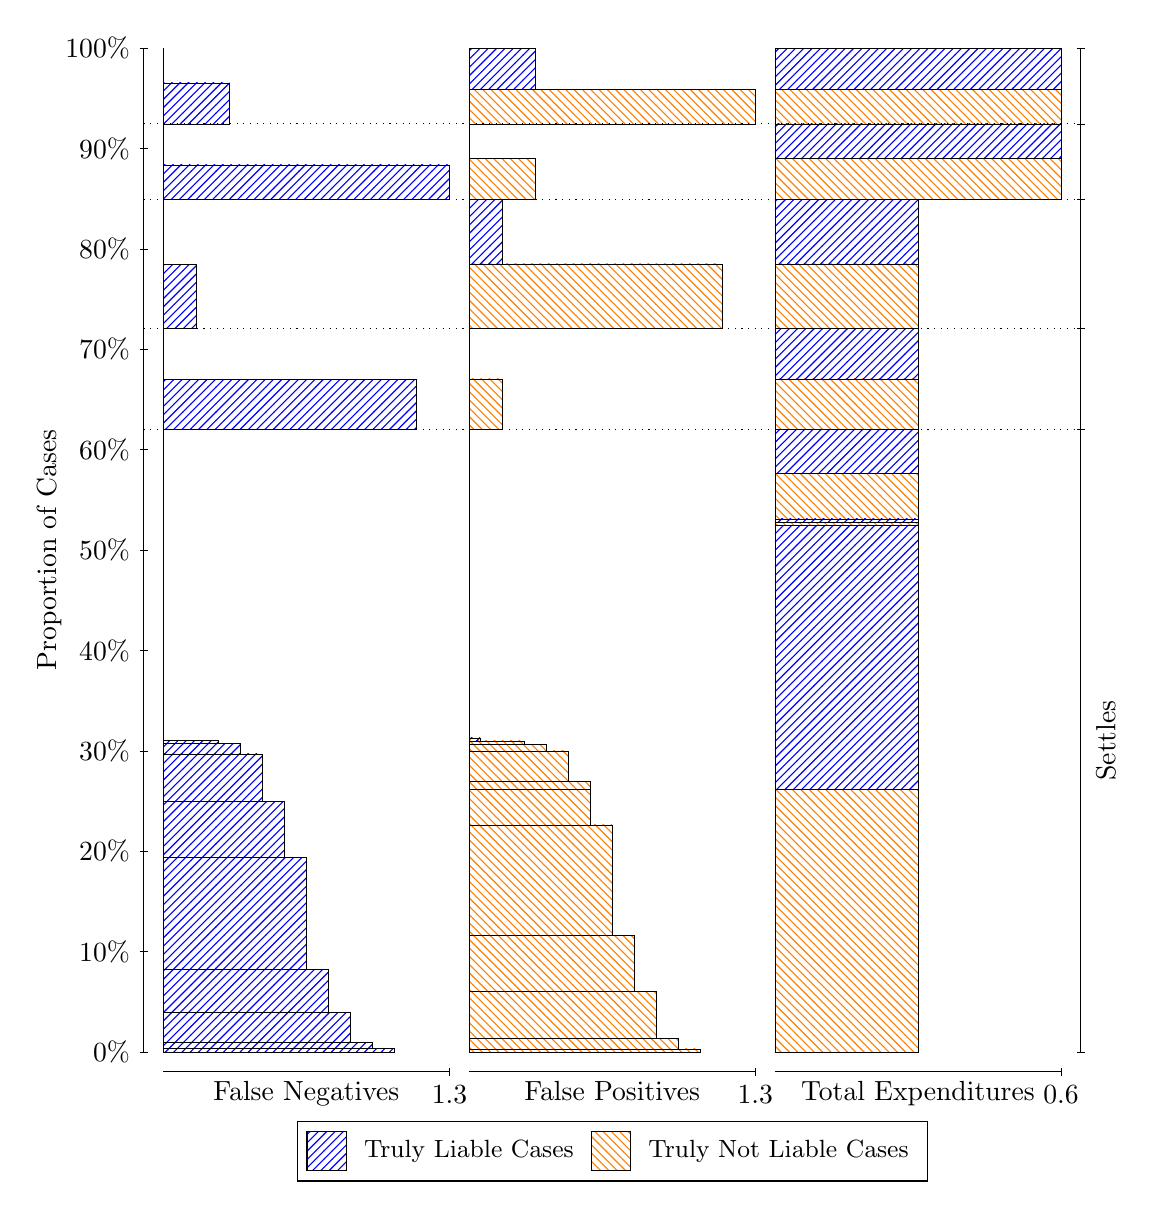
\begin{tikzpicture}
\draw[black, very thin] (1.5,1.75) -- (1.5,14.5);
\node[rotate=90, anchor=center] at (0.3, 8.125) {Proportion of Cases};
\draw[black, very thin] (1.45,1.75) -- (1.55,1.75);
\node[anchor=east] at (1.45, 1.75) {0\%};
\draw[black, very thin] (1.45,3.025) -- (1.55,3.025);
\node[anchor=east] at (1.45, 3.025) {10\%};
\draw[black, very thin] (1.45,4.3) -- (1.55,4.3);
\node[anchor=east] at (1.45, 4.3) {20\%};
\draw[black, very thin] (1.45,5.575) -- (1.55,5.575);
\node[anchor=east] at (1.45, 5.575) {30\%};
\draw[black, very thin] (1.45,6.85) -- (1.55,6.85);
\node[anchor=east] at (1.45, 6.85) {40\%};
\draw[black, very thin] (1.45,8.125) -- (1.55,8.125);
\node[anchor=east] at (1.45, 8.125) {50\%};
\draw[black, very thin] (1.45,9.4) -- (1.55,9.4);
\node[anchor=east] at (1.45, 9.4) {60\%};
\draw[black, very thin] (1.45,10.675) -- (1.55,10.675);
\node[anchor=east] at (1.45, 10.675) {70\%};
\draw[black, very thin] (1.45,11.95) -- (1.55,11.95);
\node[anchor=east] at (1.45, 11.95) {80\%};
\draw[black, very thin] (1.45,13.225) -- (1.55,13.225);
\node[anchor=east] at (1.45, 13.225) {90\%};
\draw[black, very thin] (1.45,14.5) -- (1.55,14.5);
\node[anchor=east] at (1.45, 14.5) {100\%};

\draw[black, very thin] (13.4,1.75) -- (13.4,14.5);
\draw[black, very thin] (13.35,1.75) -- (13.45,1.75);
\node[anchor=west] at (13.35, 1.75) {};
\draw[black, very thin] (13.35,9.6593) -- (13.45,9.6593);
\node[anchor=west] at (13.35, 9.6593) {};
\draw[black, very thin] (13.35,10.935) -- (13.45,10.935);
\node[anchor=west] at (13.35, 10.935) {};
\draw[black, very thin] (13.35,12.574) -- (13.45,12.574);
\node[anchor=west] at (13.35, 12.574) {};
\draw[black, very thin] (13.35,13.537) -- (13.45,13.537);
\node[anchor=west] at (13.35, 13.537) {};
\draw[black, very thin] (13.35,14.5) -- (13.45,14.5);
\node[anchor=west] at (13.35, 14.5) {};

\draw[black, very thin, pattern color=blue, pattern=north east lines] (1.75,1.75) rectangle (4.6846,1.7909);
\draw[black, very thin, pattern color=blue, pattern=north east lines] (1.75,1.7909) rectangle (4.4051,1.8719);
\draw[black, very thin, pattern color=blue, pattern=north east lines] (1.75,1.8719) rectangle (4.1256,2.2525);
\draw[black, very thin, pattern color=blue, pattern=north east lines] (1.75,2.2525) rectangle (3.8462,2.8027);
\draw[black, very thin, pattern color=blue, pattern=north east lines] (1.75,2.8027) rectangle (3.5667,4.2194);
\draw[black, very thin, pattern color=blue, pattern=north east lines] (1.75,4.2194) rectangle (3.2872,4.9366);
\draw[black, very thin, pattern color=blue, pattern=north east lines] (1.75,4.9366) rectangle (3.0077,5.5364);
\draw[black, very thin, pattern color=blue, pattern=north east lines] (1.75,5.5364) rectangle (2.7282,5.6696);
\draw[black, very thin, pattern color=blue, pattern=north east lines] (1.75,5.6696) rectangle (2.4487,5.7097);
\draw[black, very thin, pattern color=orange, pattern=north west lines] (1.75,5.7097) rectangle (1.75,9.6593);
\draw[black, very thin, pattern color=blue, pattern=north east lines] (1.75,9.6593) rectangle (4.9641,10.295);
\draw[black, very thin, pattern color=orange, pattern=north west lines] (1.75,10.295) rectangle (1.75,10.935);
\draw[black, very thin, pattern color=blue, pattern=north east lines] (1.75,10.935) rectangle (2.1692,11.751);
\draw[black, very thin, pattern color=orange, pattern=north west lines] (1.75,11.751) rectangle (1.75,12.574);
\draw[black, very thin, pattern color=blue, pattern=north east lines] (1.75,12.574) rectangle (5.3833,13.016);
\draw[black, very thin, pattern color=orange, pattern=north west lines] (1.75,13.016) rectangle (1.75,13.537);
\draw[black, very thin, pattern color=blue, pattern=north east lines] (1.75,13.537) rectangle (2.5885,14.058);
\draw[black, very thin, pattern color=orange, pattern=north west lines] (1.75,14.058) rectangle (1.75,14.5);
\draw[black, very thin, pattern color=orange, pattern=north west lines] (5.6333,1.75) rectangle (8.5679,1.7895);
\draw[black, very thin, pattern color=orange, pattern=north west lines] (5.6333,1.7895) rectangle (8.2885,1.9224);
\draw[black, very thin, pattern color=orange, pattern=north west lines] (5.6333,1.9224) rectangle (8.009,2.5185);
\draw[black, very thin, pattern color=orange, pattern=north west lines] (5.6333,2.5185) rectangle (7.7295,3.2271);
\draw[black, very thin, pattern color=orange, pattern=north west lines] (5.6333,3.2271) rectangle (7.45,4.6342);
\draw[black, very thin, pattern color=orange, pattern=north west lines] (5.6333,4.6342) rectangle (7.1705,5.0833);
\draw[black, very thin, pattern color=orange, pattern=north west lines] (5.6333,5.0833) rectangle (7.1705,5.1884);
\draw[black, very thin, pattern color=orange, pattern=north west lines] (5.6333,5.1884) rectangle (6.891,5.5741);
\draw[black, very thin, pattern color=orange, pattern=north west lines] (5.6333,5.5741) rectangle (6.6115,5.657);
\draw[black, very thin, pattern color=orange, pattern=north west lines] (5.6333,5.657) rectangle (6.3321,5.6996);
\draw[black, very thin, pattern color=blue, pattern=north east lines] (5.6333,5.6996) rectangle (5.7731,5.7396);
\draw[black, very thin, pattern color=blue, pattern=north east lines] (5.6333,5.7396) rectangle (5.6333,9.6593);
\draw[black, very thin, pattern color=orange, pattern=north west lines] (5.6333,9.6593) rectangle (6.0526,10.299);
\draw[black, very thin, pattern color=blue, pattern=north east lines] (5.6333,10.299) rectangle (5.6333,10.935);
\draw[black, very thin, pattern color=orange, pattern=north west lines] (5.6333,10.935) rectangle (8.8474,11.758);
\draw[black, very thin, pattern color=blue, pattern=north east lines] (5.6333,11.758) rectangle (6.0526,12.574);
\draw[black, very thin, pattern color=orange, pattern=north west lines] (5.6333,12.574) rectangle (6.4718,13.094);
\draw[black, very thin, pattern color=blue, pattern=north east lines] (5.6333,13.094) rectangle (5.6333,13.537);
\draw[black, very thin, pattern color=orange, pattern=north west lines] (5.6333,13.537) rectangle (9.2667,13.979);
\draw[black, very thin, pattern color=blue, pattern=north east lines] (5.6333,13.979) rectangle (6.4718,14.5);
\draw[black, very thin, pattern color=orange, pattern=north west lines] (9.5167,1.75) rectangle (11.333,5.0833);
\draw[black, very thin, pattern color=blue, pattern=north east lines] (9.5167,5.0833) rectangle (11.333,8.4371);
\draw[black, very thin, pattern color=orange, pattern=north west lines] (9.5167,8.4371) rectangle (11.333,8.4797);
\draw[black, very thin, pattern color=blue, pattern=north east lines] (9.5167,8.4797) rectangle (11.333,8.5206);
\draw[black, very thin, pattern color=orange, pattern=north west lines] (9.5167,8.5206) rectangle (11.333,9.0943);
\draw[black, very thin, pattern color=blue, pattern=north east lines] (9.5167,9.0943) rectangle (11.333,9.6593);
\draw[black, very thin, pattern color=orange, pattern=north west lines] (9.5167,9.6593) rectangle (11.333,10.299);
\draw[black, very thin, pattern color=blue, pattern=north east lines] (9.5167,10.299) rectangle (11.333,10.935);
\draw[black, very thin, pattern color=orange, pattern=north west lines] (9.5167,10.935) rectangle (11.333,11.758);
\draw[black, very thin, pattern color=blue, pattern=north east lines] (9.5167,11.758) rectangle (11.333,12.574);
\draw[black, very thin, pattern color=orange, pattern=north west lines] (9.5167,12.574) rectangle (13.15,13.094);
\draw[black, very thin, pattern color=blue, pattern=north east lines] (9.5167,13.094) rectangle (13.15,13.537);
\draw[black, very thin, pattern color=orange, pattern=north west lines] (9.5167,13.537) rectangle (13.15,13.979);
\draw[black, very thin, pattern color=blue, pattern=north east lines] (9.5167,13.979) rectangle (13.15,14.5);
\draw[black, dotted] (1.5,9.6593) -- (13.4,9.6593);
\draw[black, dotted] (1.5,10.935) -- (13.4,10.935);
\draw[black, dotted] (1.5,12.574) -- (13.4,12.574);
\draw[black, dotted] (1.5,13.537) -- (13.4,13.537);
\draw[black, very thin] (1.75,1.5) -- (5.3833,1.5);
\node[anchor=north] at (3.5667, 1.5) {False Negatives};
\draw[black, very thin] (5.3833,1.45) -- (5.3833,1.55);
\node[anchor=north] at (5.3833, 1.45) {1.3};

\draw[black, very thin] (5.6333,1.5) -- (9.2667,1.5);
\node[anchor=north] at (7.45, 1.5) {False Positives};
\draw[black, very thin] (9.2667,1.45) -- (9.2667,1.55);
\node[anchor=north] at (9.2667, 1.45) {1.3};

\draw[black, very thin] (9.5167,1.5) -- (13.15,1.5);
\node[anchor=north] at (11.333, 1.5) {Total Expenditures};
\draw[black, very thin] (13.15,1.45) -- (13.15,1.55);
\node[anchor=north] at (13.15, 1.45) {0.6};

\node[black, centered, rotate=90] at (13.72, 5.7046) {Settles};





\draw (7.449999999999999,1.5) node[draw=none] (baseCoordinate) {};
\begin{scope}[align=center]
        \matrix[scale=0.5, draw=black, below=0.5cm of baseCoordinate, nodes={draw}, column sep=0.1cm]{
            \node[rectangle, draw, minimum width=0.5cm, minimum height=0.5cm, pattern=north east lines, pattern color=blue] {}; &
            \node[draw=none, font=\small] (B) {Truly Liable Cases}; &
            \node[rectangle, draw, minimum width=0.5cm, minimum height=0.5cm, pattern=north west lines, pattern color=orange] {}; &
            \node[draw=none, font=\small] (B) {Truly Not Liable Cases}; \\
            };
\end{scope}

\end{tikzpicture}
\end{document}